\section{Probabilistic Traffic Monitoring}

%TODO: error rate?

\subsection{Overview}

\paragraph{Why Monitor Traffic}
Traffic monitoring can be used to detect anomalies (e.g. volume-based attacks such as a DoS or breaches of quality of service agreements) and to manage the network (usage-based pricing, traffic engineering, etc.).

Performed on a flow-based granularity. Flow = (Src IP, Dst IP, Src Port, Dst Port, Protocol). Also, IPv6 has an explicit flow label.

Difficult since there's so much traffic (and it grows fast) and packets needs to be processed in an extremely efficient manner.

\paragraph{Probabilistic Traffic Monitoring}
Trade accuracy (low bias) / precision (low variance) for efficiency by estimating traffic statistics based on actual traffic. 

\subsection{Measuring Flows}

\paragraph{General-Purpose Measurements (NetFlow)}
Standard NetFlow samples every packet, sampled NetFlow samples every k-th packet. It keeps a flow entry for each flow that counts the number of samples packets and bytes which is updated for every sample. To estimate the number of packets and bytes of a flow, the recorded values are multiplied by k.

\begin{figure}[h]
	\centering
	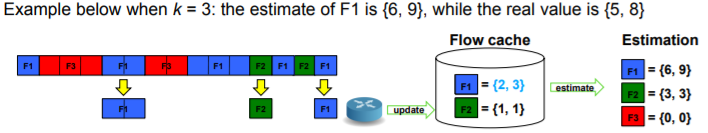
\includegraphics[scale=0.8]{images/917-netflow.PNG}
	\caption{Sampled NetFlow with k = 3.}
	\label{fig:netflow}
\end{figure}

Simple to implement and reduces the processing time but might be a memory overhead since there is one entry per flow in the worst case. The estimates are imprecise, especially for short-lived flows (most precise for flows sending many small packets). To solve imprecision, only focus on a specific traffic information instead of general purpose (e.g. only large flows as below, etc.)

\paragraph{Large Flows}
Flows that take up a given threshold of link capacity. E.g. hypergiants that generate 30\% of all Internet traffic. Less than 1\% of flows account for more than 90\% of traffic volume. It is easy to identify them (without keeping per-flow state on routers) because their number is much smaller than overall flows.

\paragraph{Sample and Hold}
Is a byte-sampling technique that takes packet size into account. Each byte is sampled with a probability $p$ so each packet with size $s$ is sampled with probability $p_s$ where $p_s = 1-(1-p)^s \approx p \cdot s$ (when $p$ is small). This reduces memory overhead since non-uniform sampling is biased toward large flows.

\begin{itemize}
    \item For each packet, check if its flow record exists. If yes, hold it (update flow entry). If no, sample it with probability $p_s$.
    \item Held / sampled packets are used to update the flow entries in the flow table (estimated number of packets and bytes per flow).
\end{itemize}

Comparison to NetFlow: Sample-and-Hold uses byte sampling instead of packet sampling. It does not over-count (but both might underestimate). Error rate of S-H is O($M^{-1}$) and of NF O($M^{-\frac{1}{2}}$) where $M$ is given memory overhead. S-H inspects all packet headers.

\paragraph{Single-Stage Filter}
Keep an array of $n$ counters. A router hashes the flow ID of an incoming packet with output $i$ in $\{1, ..., n\}$ and increases $i$-th counter. Flow is considered large if its counter value surpasses a threshold. To reduce false positives, use multiple filters in parallel.

\paragraph{Multistage Filter}
The above but with multiple filters in parallel, with each stage using a different independent hash function. Flow is large if all associated counter values surpass a threshold.

Uses fixed memory resources, no false negatives and low false positives (FP rate decreases exponentially in the number of stages).

\paragraph{Finding Frequent Items}
Find items (= packets) with a frequency that surpass chosen threshold (= large flow). See below for different kinds of algorithms.

\paragraph{Majority Algorithm}
Keep one item \textit{kept item} and one counter.

\textbf{First pass} For each new item: if counter equals to 0, \textit{kept item} is new item, increase counter, else if new item is same as \textit{kept item}, increase counter, else decrease counter.

\textbf{Second pass} Test the last \textit{kept item} to see if it is actually the one with >50\% frequency (majority).

\paragraph{MG-Algorithm}
Generalization of Majority Algorithm. Find all items that appear in a stream of $m$ items more than $k$ times with no false negatives and with limited space $n = \frac{m}{k} - 1$ counters. Needs a second pass to eliminate false positives (e.g. c in example).

\begin{figure}[h]
	\centering
	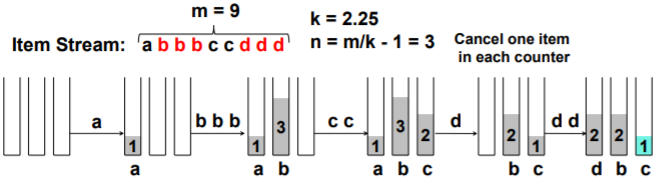
\includegraphics[scale=0.8]{images/917-mg.PNG}
	\caption{MG-algorithm.}
	\label{fig:mg}
\end{figure}

\paragraph{EARDet Algorithm}
Modifies the MG-Algorithm by switching number of packets with packet size and therefore increasing counter by size instead of number. Idle periods are replaced by virtual flows of a specific packet size (low-bandwidth threshold, e.g. idle period of 6 divided into two times 3 if THL is 3).

No false negatives for large flows and no false positives for small flows (if a certain threshold is surpassed by one of the items in the counter, it is frequent) - there is an ambiguity region between low-bandwidth and high-bandwidth threshold. Deterministic (keeps performance regardless of input traffic / attack pattern). Relatively small storage cost but many counters are needed. Con: per-packet counter is an expensive operation.

\begin{figure}[h]
	\centering
	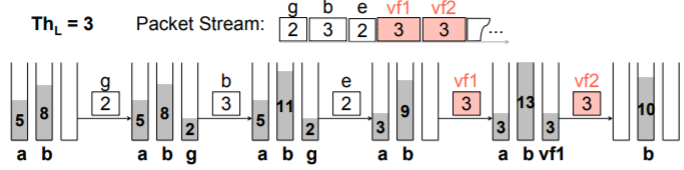
\includegraphics[scale=0.8]{images/917-eardet.PNG}
	\caption{EARDet algorithm.}
	\label{fig:eardet}
\end{figure}


\subsection{Finding Duplicates}

\paragraph{Problem}
Identify if an element is a duplicate without storing all previous elements. A Bloom Filter provides a probabilistic data structure for set membership testing.

\paragraph{Bloom Filter}
Start with bit vector $V$ that has $m$ bits and an initial value of 0. For each inserted element $e$, compute $k$ hash functions $h_i = H_i(e)$ where $0 < h_i \leq m$ and set all bits $V[h_i] = 1$. To test if an element $e'$ has already been seen, recompute all $k$ hash functions and check all $V[h_i]$, if all bits are 1, the element has been seen before.

No false negatives and constant time insertion / test. The more elements are inserted, the higher the probability of a false positive (reset filter, no more FN guarantee). Constant bits per element given FP rate (but still O(n) memory overhead).

%TODO: duplicates in practice

\begin{figure}[h]
	\centering
	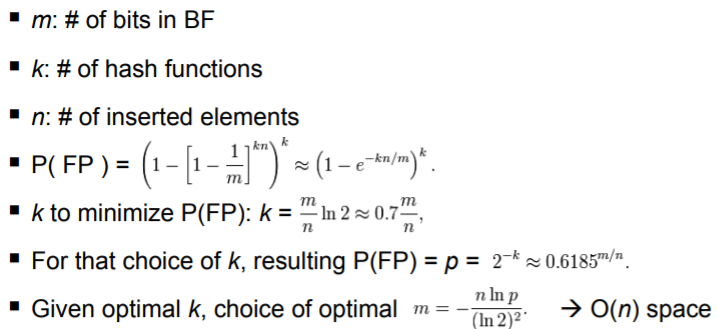
\includegraphics[scale=0.6]{images/917-bloom.PNG}
	\caption{Bloom Filter parameters.}
	\label{fig:bloom}
\end{figure}

\subsection{Estimate Number of Flows}

\paragraph{Probabilistic Counting}
See Figure \ref{fig:counting}. Problems: minimum can have very large variance and therefore this is not robust. An attacker controlling only one input can bias the estimation.

Proposal by Bar-Yossef et al.: keep track of the $k$ smallest hash values, expectation value of $k$-th smallest value is $\frac{k}{(n+1)}$ which has smaller variance. Estimate with $k$-th smallest value $v_k$ seen so far: $n \approx \frac{k}{v_k} - 1$.

Additionally, use sampling to reduce overhead induced by hashing.

\begin{figure}[h]
	\centering
	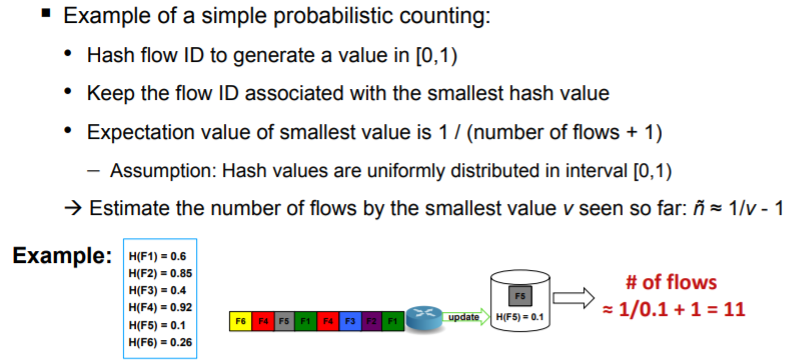
\includegraphics[scale=0.6]{images/917-counting.PNG}
	\caption{Probabilistic counting.}
	\label{fig:counting}
\end{figure}

%TODO: tm vs intrusion detection, challenges
